\section{The Sphere Packing Problem}

The Sphere Packing problem is a classical optimsation problem in mathematics. The problem can be formulated as follows.

\begin{boxproblem}[The Sphere Packing Problem in Dimensinon $n$]\label{Ch1:Prob:SpherePacking_n}
    Given some $n \in \N$, what is the densest possible non-overlapping arrangement of $n$-spheres of equal radius in $\R^n$?
\end{boxproblem}

Despite its rather straightforward formulation, \Cref{Ch1:Prob:SpherePacking_n} is notoriously difficult to solve. Indeed, one obvious question that arises when one looks at the problem statement is how one might define the concept of density. It turns out that the definition is slightly unwieldy, though introducing a periodicity assumption on the sphere packing whose density one wishes to find considerably simplifies this problem.

A key challenge in solving the sphere packing problem in dimension $n$ is the fact that proceeding inductively is not always helpful: `stacking' the optimal $n$-dimensional sphere packing onto itself is not guaranteed to yield the optimal sphere packing in $n + 1$ dimensions.~\cite{CohnOnViazovskaICM}. In fact, this appraoch is known to fail in dimensions as low as $10$~\cite{CohnOnViazovskaAMS}. This is not obvious, not least because the approach does, in fact, succeed in the visualisable dimensions of $1$, $2$ and $3$.

The $1$-dimensional case is uninteresting. Visually, one can easily see that the densest possible arrangement of disjoint intervals of the form $\parenth{-r, r}$ on the real line consists of intervals centred at all points $2rm$ for $m \in \Z$. Indeed, one can fix $r$ to be $\frac{1}{2}$ by rescaling the real line. The optimal packing therefore consists of open intervals of unit length centred at points on the lattice $\Z \subset \R$.

\begin{figure}[htb]
    \centering
    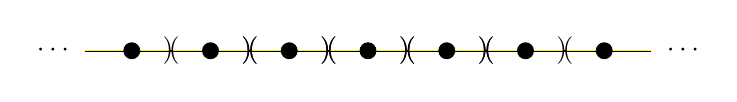
\begin{tikzpicture}
        \draw[step=1, black, thick] (-3.6, 0) -- (3.6, 0);
        \draw[yellow] (-3.6, 0) -- (-2.51, 0);
        \draw[yellow] (2.51, 0) -- (3.6, 0);
        \foreach \x in {-2, -1, 0, 1, 2} {
            \draw[yellow] (\x - 0.49, 0) -- (\x + 0.49, 0);
            \node at (\x - 0.5, 0) {$)\!($};
            \node at (\x + 0.5, 0) {$)\!($};
            \draw[fill=black] (\x, 0) circle (0.1);
        }
        \foreach \x in {-4, 4} {
            \node at (\x,0) {$\cdots$};
        }
        \draw[fill=black] (-3, 0) circle (0.1);
        \draw[fill=black] (3, 0) circle (0.1);
    \end{tikzpicture}
    \caption{The $\Z$ lattice packing in dimension $1$.}
    \label{Ch1:Fig:Z_Lattice_Packing_1D}
\end{figure}

Rescaling gives us a powerful---if straightforward---simplification of the sphere packing problem where we can fix the radius of the spheres to a convenient value. Indeed, we only mention rescaling explicitly because it needs to be explicitly dealt with when formalising the problem. We will resume this discussion in \todo{ADD REFERENCE}. For now, we will take for granted the fact that rescaling does not affect the density of a sphere packing, meaning that we can talk about optimal sphere packings without worrying about the radius of the spheres in question. Bearing in mind that the spheres must all have the same radius, as per the statement of \Cref{Ch1:Prob:SpherePacking_n}, we will henceforth describe sphere packings simply by describing the points at which the spheres are centred.

The sphere packing problem in dimension $2$, also known as the circle packing problem, turns out to be more interesting. A reasonable strategy for finding the densest packing is to `stack' the $\Z$ lattice packing from dimension $1$ onto itself in some manner, but the question remains as to exactly how this should be done. `Stacking' it onto itself would involve extending the lattice $\Z \subset \R \subset \R^2$ into a lattice in $\R^2$ by extending the $\R$-basis $\set{\parenth{1, 0}}$ of $\R$ (viewed as a subspace of $\R^2$) to an $\R$-basis of $\R^2$, and taking its $\Z$-span.

One natural way of doing this is to extend the lattice $\Z \subset \R$ to the lattice $\Z^2 \subset \R^2$ consisting of points with integer coordinates. This corresponds to the natural extension of $\set{\parenth{1, 0}}$ to the standard $\R$-basis $\set{\parenth{1, 0}, \parenth{0, 1}}$ of $\R^2$. See \Cref{Ch1:Subfig:Z2_lattice_packing_2D}.

Unfortunately, this packing turns out to be sub-optimal \todo{Do we want to add the density?}. A better candidate is the $A_2$ lattice packing, corresponding to the extension of $\set{\parenth{1, 0}}$ to the $A_2$ root basis $\set{\parenth{1, 0}, \parenth{-\frac{1}{2}, \frac{\sqrt{3}}{2}}}$. See \Cref{Ch1:Subfig:A2_lattice_packing_2D}. This packing is sometimes referred to as the honeycomb packing due to the hexagonal arrangement of centres.

It is well-known that the honeycomb packing is \textit{optimal} in $\R^2$. What this means is that no circle packing has a density greater than that of the honeycomb packing. The original proof of this fact is attributed to Thue \cite{Thue}, but there have since been several arguments establishing its validity. One approach based on an idea of Rogers's that does not require particularly sophisticated mathematical tools was outlined by Hales in \cite{CannonHoney}. Indeed, in \Cref{Ch1:fig:Circle_Packings_2D}, we can intuitively see that the $A_2$ packing is denser than the $\Z^2$ packing. While the comparison does not establish the optimality of the $A_2$ packing, it is admittedly not wholly surprising, from looking at \Cref{Ch1:fig:Circle_Packings_2D}, that the density of the $A_2$ packing cannot be improved.

\begin{figure}[htb]
    \centering
    \begin{subfigure}{0.48\linewidth}
        \centering
        \begin{tikzpicture}[scale=1.25]
            \drawplane
            \foreach \x in {-2, -1, 0, 1, 2} {
                \foreach \y in {-2, -1, 0, 1, 2} {
                    \latticecircle{\x}{\y}
                }
            }
            \draw[->, color=brown, thick] (0,0) -- (1,0) node[anchor=north] {$\parenth{1, 0}$};
            \draw[->, color=brown, thick] (0,0) -- (0,1) node[anchor=east] {$\parenth{0, 1}$};
        \end{tikzpicture}
        \subcaption{The $\Z^2$ lattice packing.}
        \label{Ch1:Subfig:Z2_lattice_packing_2D}
    \end{subfigure}
    \begin{subfigure}{0.48\linewidth}
        \centering
        \begin{tikzpicture}[scale=1.25]
            \drawplane
            \clip (-2.5, -2.5) rectangle ++(5, 5);
            \foreach \x in {-4, -3, -2, -1, 0, 1, 2, 3, 4} {
                \foreach \y in {-3, -2, -1, 0, 1, 2, 3} {
                    \latticecircle{\x - \y * 0.5}{\y * 0.8660254038}
                }
            }
            \draw[->, color=brown, thick] (0,0) -- (1,0) node[anchor=north] {$\parenth{1, 0}$};
            \draw[->, color=brown, thick] (0,0) -- (-0.5,0.8660254038) node[anchor=south east] {$\parenth{-\frac{1}{2}, \frac{\sqrt{3}}{2}}$};
        \end{tikzpicture}
        \subcaption{The $A_2$ lattice packing.}
        \label{Ch1:Subfig:A2_lattice_packing_2D}
    \end{subfigure}
    \caption{Circle packings covering the square $\setst{\parenth{x, y} \subset \R^2}{-2.5 \leq x, y \leq 2.5}$.}
    \label{Ch1:fig:Circle_Packings_2D}
\end{figure}
